\documentclass[a4paper]{article}
\usepackage[utf8]{inputenc}
\usepackage[russian]{babel}
\usepackage[T2]{fontenc}
\usepackage[warn]{mathtext}
\usepackage{graphicx}
\usepackage[left=30mm, top=20mm, right=20mm, bottom=20mm, footskip=10mm]{geometry}


\graphicspath{ {images/} }
\usepackage{multicol}
\setlength{\columnsep}{2cm}


\begin{document}

\begin{titlepage}
	\centering
	\vspace{5cm}
	{\scshape\LARGE Московский физико-технический институт \par}
	\vspace{4cm}
	{\scshape\Large Лабораторная работа \par}
	\vspace{1cm}
	{\huge\bfseries Получение и измерение вакуума \par}
	\vspace{1cm}
	\vfill
\begin{flushright}
	{\large выполнила студентка 653 группы ФФКЭ}\par
	\vspace{0.3cm}
	{\LARGE Карпова Татьяна}
\end{flushright}
	

	\vfill

% Bottom of the page
	Долгопрудный, 2017 г.
\end{titlepage}

\section{Цель работы}
\begin{enumerate}
    \item Измерение объёмов форвакуумной и высоковакуумной частей установки
    \item Определение скорости откачки системы в стационарном режиме, а также по ухудшению и улучшению вакуума
\end{enumerate}

\section{В работе используются:}
\begin{itemize}
    \item вакуумная установка
    \item масляный, термопарный и ионизационный вакуумметры
    \item форвакуумный и диффузионный насосы
\end{itemize}

\section{Экспериментальная установка}

По степени разрежения вакуумные установки принято делить на три класса: 1) низковакуумные — до $10^-^2$–$10^-^3$ торр; 2) высоковакуумные — $10^-^4$–$10^-^7$ торр; 3) установки сверхвысокого вакуума — $10^-^8$–$10^-^11$ торр. В данной работе изучаются традиционные методы откачки механическим форвакуумным насосом до давления $10^-^2$ торр и диффузионным масляным насосом до давления
$10^-^5$ торр, а также методы измерения вакуума в этом диапазоне.

\begin{figure}[h]
    \centering
    \includegraphics[width=\textwidth]{setup.PNG}
    \caption{Схема экспериментальной установки}
    \label{fig:vac}
\end{figure}

Установка изготовлена из стекла и состоит из форвакуумного баллона (ФБ), высоковакуумного диффузионного насоса (ВН), высоковакуумного баллона (ВБ), масляного (М) и ионизационного (И) манометров, термопарных манометров (М1 и M2), форвакуумного насоса (ФН) и соединительных кранов
К1, К2, ..., К6 (рис. 1). Кроме того, в состав установки входят: вариатор
(автотрансформатор с регулируемым выходным напряжением), или реостат
и амперметр для регулирования тока нагревателя диффузионного насоса.

\section{Теоретические положения}
\subsection{Процесс откачки}
Производительность насоса определяется скоро-
стью откачки W (л/с): W — это объем газа, удаляемого из сосуда при
данном давлении за единицу времени. Скорость откачки форвакуум-
ного насоса равна емкости воздухозаборной камеры, умноженной на
число оборотов в секунду. \par
Обозначим через Qд количество газа, десорбирующегося с поверхности откачиваемого объема в единицу времени, через Qи — количество газа, проникающего в единицу времени в этот объем извне — через течи. Будем считать, что насос обладает скоростью откачки W и в то же время сам является источником газа; пусть Qн — поток газа, поступающего из насоса
назад в откачиваемую систему. Будем измерять количество газа Qд, Qн и Qи в единицах PV (легко видеть, что это произведение с точностью до множителя $RT/\mu$ равно массе газа). Основное уравнение, описывающее процесс откачки, имеет вид
\begin{center}
$−VdP = (PW - Q$д$ - Q$н$ - Q$и$)dt$.
\end{center}
При достижении предельного вакуума 
\begin{center}
$\frac{dP}{dt}=0$,
\end{center}
поэтому
\begin{center}
$P$пр$W =Q$д $ + Q$н $ + Q$и.
\end{center}

Формула, выражающая скорость откачки через предельный вакуум:
\begin{center}
$W = \sum Q_i / P$пр.
\end{center}

Считая постоянными потоки газа и скорость откачки, интегрируем первое уравнение и получаем
\begin{center}
$P - P$пр $= (P_0 - P$пр $) exp(-\frac{W}{V}t)$
\end{center}
При начальном давлении $P_0$ значительно большем чем $P$пр, имеем
\begin{center}
$P = P_0 exp(-\frac{W}{V}t) + P$пр.
\end{center}

Скорость откачки системы зависит от характеристик насоса, перепада давлений, а также от пропускной способности трубопроводов. Практическое правило заключается в том, что диаметры соединительных трубок не очень существенны в форвакуумной части установки и крайне важны в высоковакуумной. Диаметр трубок в этой части должен быть не меньше, чем диаметр самого насоса.

\subsection{Течение газа через трубу}

Характер течения газа существенно зависит от соотношения между размерами системы и длиной свободного пробега молекул. При атмосферном давлении
и даже при понижении давления до форвакуумного длина свободного пробега меньше диаметра трубок и течение откачиваемого газа определяется его вязкостью, т. е. взаимодействием его молекул. При переходе к высокому
вакууму столкновения молекул между собой начинают играть меньшую роль, чем соударения со стенками. \par
Для количества газа, протекающего через трубу в условиях высокого вакуума, справедлива формула
\begin{center}
$\frac{d(PV)}{dt} = \frac{4}{3}r^3 \sqrt{\frac{2\pi RT}{\mu}}\frac{P_2-P_1}{L}$.
\end{center}
Применим эту формулу к случаю, когда труба соединяет установку с насосом. \par
Пренебрежём давлением $P_1$ у конца, обращённого к насосу. Будем измерять количество газа, покидающего установку при давлении P = $P_2$. Пропускная способность трубы
$C = (\frac{dV}{dt}) = \frac{4}{3}\frac{r^3}{L}\sqrt{\frac{2\pi RT}{\mu}}$
Пропускная способность зависит от радиуса трубы в
третьей степени и обратно пропорциональна ее длине. \par
При расчете вакуумных систем нужно принимать во внимание также пропускную способность отверстий, например, в кранах. Для них имеется формула
\begin{center}
$\nu = \frac{1}{4}Sn\bar v$,
\end{center}
где $\nu$ — число молекул, вылетающих из отверстия в вакуум в единицу
времени, $S$ — площадь отверстия, $n$ — концентрация молекул перед отверстием, $\bar v$ — средняя скорость молекул газа. \par
С другой стороны, $\nu = dN/dt$, $N = PV/kT$, $n=P/kT$, и аналогично формуле для количества газа, покидающего установку при давлении P, получается пропускная способность отверстия
\begin{center}
$C = (\frac{dV}{dt})=S\frac{\bar v}{4}$.
\end{center}
Для воздуха при комнатной температуре $\bar v$/4 = 110 м/с = 11 л/с·см2

\section{Ход работы}

\subsection{Определение объёма форвакуумной и высоковакуумной частей установки}

\begin{enumerate}
    \item Проверим, что открыт кран К4. Откроем все краны, крое К1 и К2. Через краны К1 и К2 впустим в установку атмосферный воздух. Закроем краны К5 и К6, при этом в кранах и соединяющем их капилляре <<запирается>> 60 $\pm$ 3 cм$^3$
    \item Закроем краны К1 и К, включим форвакуумный насос и дадим ему откачать себя примерно 1-2 минуты. Краном К2 подключим установку к форвакуумному насосу и откачаем установку до давления порядка $10^-^2$ торр. Давление измеряется вакуумметром ВТ-2, соединённым с лампой М1. После того как давление достигло необходимого порядка, отсоединим систему от насоса, закрыв кран К2.
    \item Закроем кран К3, отсоединив высоковакуумную часть установки от форвакуумной. Подготовим к измерениям масляный манометр, закрыв кран К4. Откроем кран К5, при этом <<запертый>> в кранах и капилляре воздух распространится по всему объёму форвакуумной части и повысит в ней давление. Это давление измерим масляным манометром, значения высоты масляных столбов занесём в таблицу 1. Зная объём <<запертого>> воздуха определим объём форвакуумной части установки по формуле
    \begin{center}
    $V = \frac{P_0 V_0}{P}$,
    \end{center}
    где $P_0$ - атмосферное давление, $V_0$ - объём <<запертого>> воздуха, $P$ - давление, измеренное масляным манометром.
    
    \item Откроем кран К3, чтобы газ заполнил также высоковакуумную часть установки. По показаниям манометра определим объём всей установки и её высоковакуумной части, занесём результаты в таблицу 1. Откроем кран К4.
    \item Измерения по пп 1-4 повторим ещё 2 раза. 
    \item Оценим погрешность измерений. Погрешность среднего значени давления, измеренного масляным барометром, оценим по формуле
    \begin{center}
        $\sigma H = \sqrt{\frac{1}{n(n-1)}\sum_{i=1}^n(H_i-\bar H)^2 \quad} $
    \end{center}
    Погрешность измерения барометром-анероидом $\sigma P_0= 100$ Па, погрешность определения объёма <<запертого>> воздуха $\sigma V_0 = 3* 10^-^6$ м$^3$. Тогда погрешность определения объёма камер будет равна (с учётом того, что     причём $\frac{\sigma P}{P}$ = $\frac{\sigma H}{H}$)
    \begin{center}
    $\sigma V = V\sqrt{(\frac{\sigma P_0}{P_0})^2+(\frac{\sigma V_0}{V_0})^2+(\frac{\sigma H}{H})^2} $,
    \end{center}

    
    \begin{table}[t]
    \centering
    \begin{center}
    \caption{Расчёт объёмов форвакуумной и высоковакуумной частей установки, объёма всей установки, погрешность измерений}
    \end{center}
    \vspace{0.1cm}
    \label{tab:my_label}
    \begin{tabular}{ |p{2.5cm}||p{1.5cm}|p{1.5cm}|p{1.5cm}|  }
 \hline
 Измерение & №1 & №2 & №3\\
\hline 

 $H_u_p$фв, мм & 223 & 223 & 223 \\
 $H_d_o_w_n$фв, мм& 402 & 403 & 402 \\
 $\triangle H$фв, мм & 179 & 180 & 179 \\
 $H_u_p$уст, мм & 259 & 259 & 260 \\
 $H_d_o_w_n$уст, мм& 360 & 360 & 360 \\
 $\triangle H$уст, мм & 101 & 101 & 100 \\
 $P$фв, Па & 1554,22 & 1562,90 & 1554,22 \\
 $P$уст, Па & 876,96 & 876,96 & 868,28 \\
 $V$фв, л & 3,899 & 3,877 & 3,899 \\
 $V$вв, л & 6,910 & 6,910 & 6,979 \\
 $V$уст, л & 3,011 & 3,033 & 3,080 \\
 \hline
\end{tabular}

\end{table}

\item Получили 
\begin{center}
Объём форвакуумной части $V$фв = 3,892 $\pm$ 0,05 л\\
Объём высоковакуумной части $V$вв = 3,041 $\pm$ 0,07 л\\
Объём всей установки $V$уст = 6,933 $\pm$ 0,05 л\\
\end{center}

\end{enumerate}
\newpage

\subsection{Получение высокого вакуума и измерение скорости откачки}

\begin{enumerate}
    \item Продолжим откачивать установку форвакуумным насосом. Включим термопарный вакуумметр ВИТ-2 и по градуировочной кривой проверим ЭДС. После того, как давление упадёт примерно до $2*10^-^2$ торр, закроем краны К5 и К6 и приступим к откачке высоковакуумной части насоса с помощью диффузионного насоса. По вакуумметру ВИТ-2 пронаблюдаем за процессом откачки высоковакуумного баллона, необходимо достигнуть давления порядка 10$^-^4$ торр, что соответствует ЭДС 10 mV. Когда стрелка прибора достигнет этого значения, закроем кран К6.
    \item Включим ионизационный вакууметр. Измерим предельное давление: его значение 2,4*10$^-^4$ торр. 
    \item Найдём скорость откачки по улучшению и ухудшению вакуума. Закроем кран К3, отключив тем самым откачку высоковакуумного баллона, и запишем ухудшение вакуума по изменению показаний ионизационного вакуумметра от времени (не более чем до 8*10$^-^4$ торр). Затем откроем кран К3 и запишем улучшение вакуума по изменению показаний микроамперметра во времени. Результаты занесём в таблицу 2.

    \begin{table}[h]
    \centering
    \begin{center}
    \caption{Изменение давления в высоковакуумном баллоне при улучшении и ухудшении вакуума в зависимости от времени}
    \end{center}
    \vspace{0.1cm}
    \label{tab:my_label}
    \begin{tabular}{ |p{0.5cm}|p{1cm}|p{0.5cm}|p{1cm}|p{0.5cm}|p{1cm}|p{0.5cm}|p{1cm}|  }
 \hline
\multicolumn{4}{|c|}{Улучшение вакуума} & \multicolumn{4}{c|}{Ухудшение вакуума} \\
 \hline
  \hline
 \multicolumn{2}{|c|}{№1} & \multicolumn{2}{c|}{№2} &
\multicolumn{2}{c|}{№1} & \multicolumn{2}{c|}{№2} \\
 \hline
t, c & P,10$^-^4$ & t, c & P,10$^-^4$ & t, c & P,10$^-^4$ & t, c & P,10$^-^4$\\
\hline 
0 & 8 & 0 & 8 & 0 & 2,4 & 0 & 2,4\\
4 & 7 & 2 & 7 & 10 & 3 & 10 & 3\\
8 & 6 & 5 & 6 & 31 & 4 & 31 & 4\\
12 & 5 & 10 & 5 & 58 & 5 & 55 & 5\\
20 & 4 & 20 & 4 & 84 & 6 & 88 & 6\\
38 & 3 & 38 & 3 & 113 & 7 & 106 & 7 \\
59 & 2,6 & 61 & 2,6 & 145 & 8 & 141 & 8\\
83 & 2,4 & 93 & 2,4 & & & &\\


 \hline
\end{tabular}

\end{table}
    \item Чтобы определить скорость откачки W системы, воспользуемся формулой
    \begin{center}
    $P - P$пр $= (P_0 - P$пр$)exp(-\frac{W}{V}t)$.
    \end{center}
    Получим формулу для исследования значений по улучшению вакуума:
    \begin{center}
    $ln(P - P$пр$) = -\frac{W}{V}t + ln(P_0 - P$пр$)$.
    \end{center}
    В этих координатах построим график зависимости давления в высоковакуумной части при улучшении вакуума от времени(сделано 2 измерения).
    
\begin{figure}[h]
    \centering
    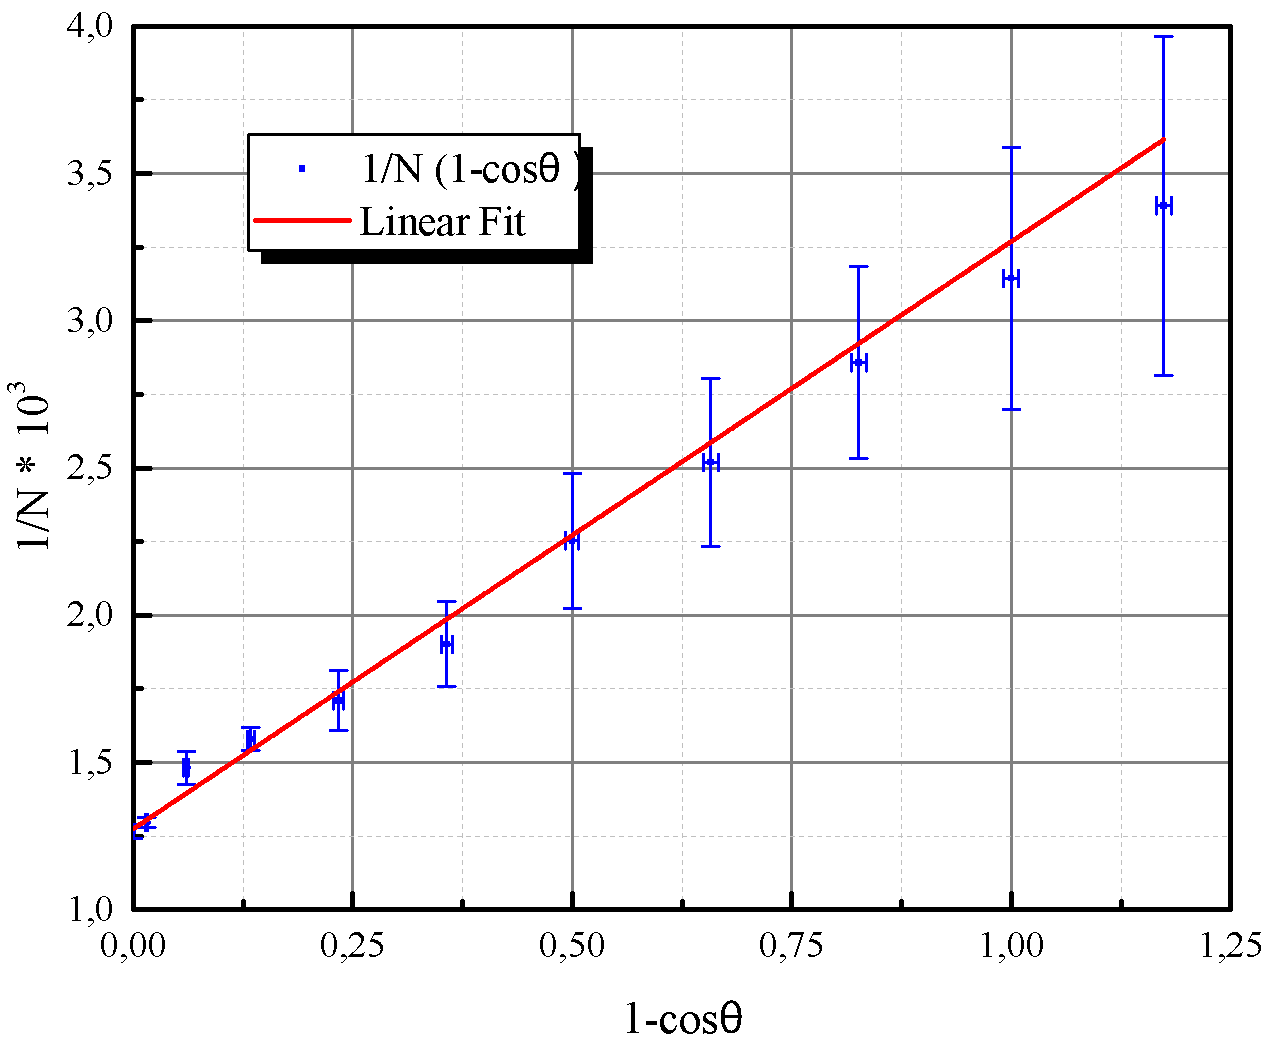
\includegraphics[width=\textwidth]{graph1.PNG}
    \caption{Зависимость давления от времени, улучшение вакуума}
    \label{fig:vac}
\end{figure}

    Коэффициент угла наклона равен -0,0552 = $-\frac{W}{V}$. Тогда, зная объём высоковакуумного баллона (часть 5.1), получаем скорость откачки системы $W = 0,1679$ л/с. Оценим по методу наименьших квадратов погрешность определения углового коэффициента:
\begin{center}
$\sigma_k = \frac{1}{\sqrt{n}}\sqrt{\frac{\langle y^2 \rangle - \langle y \rangle ^2}{\langle x^2 \rangle - \langle x \rangle ^2} - k^2} = 0,024$,
\end{center}

и погрешность определённого значения скорости откачки диффузионного насоса будет равна

\begin{center}
$\sigma W = W\sqrt{(\frac{\sigma k}{k})^2+(\frac{\sigma V}{V})^2} = 0,005$
\end{center}
Полученная скорость откачки диффузионного насоса:
\begin{center}
$W = 16,79 \pm 0,5 * 10^-^2$ л/с
\end{center}

\item Оценим величину потока $Q$н. Воспользуемся уравнением 
\begin{center}
$V_B_B dP = (Q$д$ + Q$и$)dt$,
\end{center}
получаем зависимость (k - коэффициент наклона прямой графика в координатах P(t))
\begin{center}
$Q$д$ + Q$и$ = k V_B_B$
\end{center}

\begin{figure}[h]
    \centering
    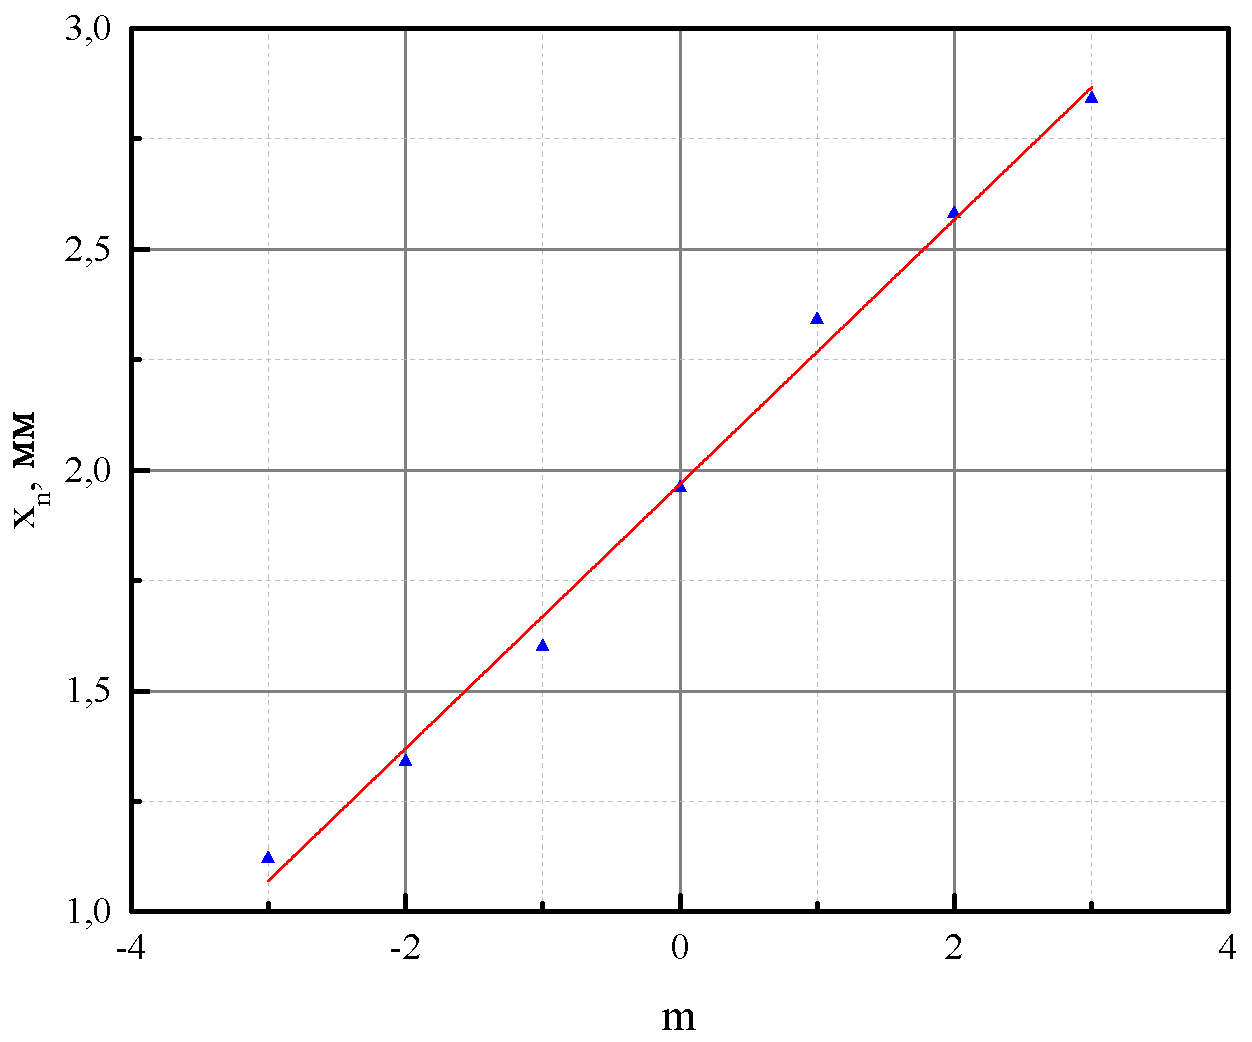
\includegraphics[width=\textwidth]{graph2.PNG}
    \caption{Зависимость давления от времени, ухудшение вакуума}
    \label{fig:vac}
\end{figure}

Зная также, что $P$пр$W = Q$д$ + Q$и$ + Q$н , получим
\begin{center}
$Q$н $= P$пр$W - k V_B_B = 28,497 * 10^-^6$ л/с
\end{center}

По графику определим $k = 3,88 * 10^-^6$, погрешность определения углового коэффициента по формуле из 5.2.4 $\sigma_k = 8,13 * 10^-^9$, величину W и её погрешность возьмём из 5.2.4, $P$пред = 2,4 * 10$^-^4$ торр. Погрешность измерения $Q$н определим по формуле
\begin{center}
$\sigma Q = \sqrt{PW((\frac{\sigma P}{P})^2+(\frac{\sigma W}{W})^2) + kV((\frac{\sigma k}{k})^2+(\frac{\sigma V}{V})^2)} = 2,082 * 10^-^6$ л/с
\end{center}

\item Откроем кран К6 и введём в прибор искусственную течь. Вакуум в установке ухудшится, измерим установившееся давление $P$уст = $P_1$ 8,8 * 10 $^-^2$ торр и давление со стороны форвакуумной части капилляра $P$2 = 4,3 * 10$^-^2$ торр. Рассчитаем производительность насоса по различию $P$уст и $P$пр. L капилляра 60 мм, r капилляра 0,45 мм.
\begin{center}
$P$уст $W = Q_1 + \frac{d(PV)_k}{dt}$, $P$пр $W = Q_1$\\
$\frac{d(PV)_k}{dt} = \frac{4}{3}r^3 \sqrt{\frac{2\pi RT}{\mu}}\frac{P_2-P_1}{L}$\\
$W = \frac{4}{3}\frac{r^3}{L}\sqrt{\frac{2\pi R T}{\mu}}\frac{P_2-P_1}{P_y - P_l_i_m} = 9,73 * 10^-^2$ л/с
\end{center}

Погрешность определения скорости откачки этим способом оценим по формуле
\begin{center}
$\sigma W = W\sqrt{9(\frac{\sigma r}{r})^2+(\frac{\sigma L}{L})^2+\frac{1}{2}(\frac{\sigma T}{T})^2+(\frac{\sigma P_2^2 + \sigma P_1^2}{(P_2-P_1)^2})+(\frac{\sigma P_y^2 + \sigma P_l_i_m^2}{(P_y-P_l_i_m)^2})} = 0,82 * 10^-^2$ л/с
\end{center}
Наибольший вклад в погрешность вносит погрешность определения радиуса капилляра, так как она входит в рабочую формулу в третьей степени. 

Сравним полученное нами значение скорости откачки со значением из п. 5.2.4

\begin{center}
$W_1 = 16,79 \pm 0,5 * 10^-^2$ л/с\\
$W_2 = 9,73 \pm 0,82 * 10^-^2$ л/с
\end{center}

Величины совпали по порядку значения, но значение скорости откачки, полученное вторым способом, оказалось меньше, чем определённое по улучшению вакуума. Скорее всего, значение, определённое первым способом, точнее (см. вывод) 
       
\end{enumerate}

\section{Вывод}

В ходе работы было проведено ознакомление с вакуумной установкой, некоторыми приборами вакуумной техники, изучены их характеристики. 
\begin{enumerate}
    \item Были определены объёмы форвакуумной и высоковакуумной частей установки. 
    \begin{center}
    \begin{center}
Объём форвакуумной части $V$фв = 3,892 $\pm$ 0,05 л\\
Объём высоковакуумной части $V$вв = 3,041 $\pm$ 0,07 л\\
Объём всей установки $V$уст = 6,933 $\pm$ 0,05 л\\
\end{center}
Эти значения соответствуют реальным (определённым глядя на исследуемые объёмы)
    \end{center}
    
    \item Был исследован принцип действия высоковакуумного диффузионного насоса, экспериментально определён поток воздуха, вытекающий через насос назад в высоковакуумную часть установки при откачке:
    \begin{center}
    $Q$н $= 28,497 \pm 2,082 * 10^-^6$ л/с
    \end{center}
    Эта величина оказалась сравнительно мала (на 4 порядка меньше) по сравнению с определённой экспериментально двумя способами скоростью откачки самого насоса
    \item Двумя способами была определена скорость откачки диффузионного насоса: по улучшению вакуума и по разности давлений при впускании в высоковакуумную часть искусственной течи и предельного давления в высоковакуумной части установки.
    Полученные результаты:
\begin{center}
$W_1 = 16,79 \pm 0,5 * 10^-^2$ л/с\\
$W_2 = 9,73 \pm 0,82 * 10^-^2$ л/с
\end{center}

     {\it Возможные причины несовпадения результатов.}
     Основная предполагаемая причина несовпадения результатов заключается в принципе работы высоковакуумных насосов. При уменьшении давления в высоковакуумной части их производительность начинает падать. Эта зависимость была исследована нами в факультетском курсе вакуумной электроники при исследовании турбомолекулярного насоса. Так как с течением времени давление в высоковакуумной части уменьшилось как минимум на порядок (с 10$^-^3$ до 10$^-^4$ торр), а эксперимент проводился около 30 минут, такое понижение производительности вполне объяснимо.
     Также могли сыграть роль следующие факторы
    \begin{itemize}
        \item в формуле для определения скорости откачки вторым способом фигурирует температура. Была взята комнатная температура, но температура воздуха в установке по факту выше: его нагревают элементы, нагревающие масло в диффузионном насосе. Эта температура достаточно велика, поэтому конечное значение скорости откачки с её учётом должно увеличиться
        \item возможные неточности при измерении длины капилляра и его радиуса
        \item могла сбиться калибровка шкалы вакуумметров на форвакууме и высоком вакууме: в процессе работы несколько раз приходилось корректировать калибровку, в конце работы этих действий произведено не было. 
    \end{itemize}
    
    Тем не менее, в ходе работы была подтверждена высокая эффективность диффузионного насоса: значение скорости откачки на 4 порядка выше, чем величина потока, возвращаемого в высоковакуумную часть установки.
\end{enumerate}


\end{document}
